A lot of times, when furries talk, they talk about their fursoñas as their ideal selves. I've found that it's more likely that their fursoñas are them at their most normal, most natural, most earnest.

It's strange that this venue seen as escapist by even its own members is basically just a means of exploring what it means to be earnest in an ironic world.

\begin{ally}
Is it?
\end{ally}
Every time I think we're living in a post-ironic world, the Internet proves me wrong.

\begin{ally}
I wouldn't know.
\end{ally}
Do you not experience irony?

\begin{ally}
A friend asks Maddy: what is irony?
\end{ally}
\end{leftcolumn}
\begin{rightcolumn*}
  \label{koan}
\noindent A friend asked Maddy: what is the importance of tension?

Maddy said: I don't know

The friend looked sad and went away.

When the friend came back, they asked: what is the importance of tension?

Maddy said: I know-

But the friend cut her off angrily and left in a huff.

Later, the friend asked Maddy: what is the importance of tension?

Maddy said: I know: I don't know

Then they sat and chatted over a cup of tea.
\newpage

\noindent A friend asked Maddy: why do you drink tea?

Maddy said: I like it. It's tasty, it makes me feel good.

The friend said: well that's dumb.

Maddy went and drank tea.

The friend asked: why do you drink tea?

Maddy said: I don't know.

The friend said: well that's dumb.

Maddy went and drank tea.

The friend asked: why do you drink tea?

Maddy said: I like it. It's tasty, it makes me feel good.

The friend laughed and clapped delightedly, and said: perfect

Then sat to drink tea with Maddy.
\newpage

\noindent A friend asked Maddy: why are you coating yourself with grease?

Maddy said: so that when I run through a field, no dirt will stick to me, and I won't get poked by thorns.

Maddy ran through the field, and wound up covered in dirt and scratches.

The friend said: better to not run.
\newpage

\noindent Maddy built a sand castle and it was washed away.

The first friend was sad about the sand castle for Maddy, and said: better to not build the sand castle and risk further sorrow.

The second friend said this was good, because Maddy saw adversity and built the castle anyway.

The third said this was good because Maddy was able to acknowledge the castle and let it pass.

A fourth said: better to have never built the castle. The sand is itself, the wave is itself, and Maddy remains.

The fifth was helping build a bigger, better sand castle.
\newpage

\noindent A friend asked Maddy: why are you nailing boards together?

Maddy said: I'm building a house to live in.

When the friend came back later, there was an awkward jumble of sticks nailed together on the ground. They said: well that was dumb.

Some time later, the friend visited Maddy and asked: why are you frowning?

Maddy said: I paid someone to build me a house, but it's round, upside down, and a mile to the east of where it should be.

The friend shrugged and said: well that was dumb

Some time later, the friend visited Maddy and found her reading on the front porch of a cozy home. They said: did you build this?

Maddy said: no, but I did my part.

The friend laughed and sat down next to Maddy to read with her.
\newpage

\begin{ally}
Are you having fun?
\end{ally}
Yes.

\begin{ally}
You know that I'm not the friend, right?
\end{ally}
I do.

\begin{ally}
Carry on.
\end{ally}
No, I'm finished for now.
\newpage

\end{rightcolumn*}
\begin{leftcolumn}
\newpage

I talk up my style as frumpcore. \emph{It's the synthesis of momcore and downtempo librarian,} I say. In reality, It's an intentionally garbage-y, thrown-together look designed to, I hope, lead onlookers' eyes to slide right off of me as unremarkable.

\begin{ally}
Ah yes, the invisible six-foot-one trans woman with purple hair. That tired old trope.
\end{ally}
While I've had fursoñas that were intended to be something better than myself --- Makyo, for a while, was dressed in a nice suit --- more often than not, they've played along similar lines.

Ranna was a gay fox, a bit pudgy, with two tails he readily admitted were an early affectation to differentiate himself from countless other foxes.

Makyo was intentionally a transfeminine vixen who didn't pass.

Maddy's a dumpy, nerdy cis girl who dresses to hide her weight.

\begin{ally}
And Madison's a dumpy, nerdy transfeminine girl who doesn't pass and dresses to hide her weight?
\end{ally}
I suppose.

\begin{ally}
You don't give yourself enough credit.
\end{ally}
Is that your department, now? Cheering me on?

\begin{ally}
I'm your ally.
\end{ally}
But not my friend.

\begin{ally}
No, but I am your ally.
\end{ally}
Fine. How do I not give myself enough credit?

\begin{ally}
Firstly, you're not as invisible as you seem and frumpcore isn't seen as that cohesive from the outside. Secondly, you pass better than you imagine. Everyone tells you that, you just can't yet hear it. Finally, you just got done writing some heavy shit after a day of worrying about work, so of course you're down on yourself. You don't want to pass, remember? You want to be visibly trans. You want to be seen as the trans psychopomp you strive to be.
\end{ally}
\ldots{}Wow.

\begin{ally}
Your very words set lie to your insecurities. Your fursoñas are yourself expressed more earnestly than you can manage in person.
\end{ally}
Thank you.

\begin{ally}
If you could become Maddy, would you?
\end{ally}
Yeah, in a heartbeat.

\begin{ally}
Why?
\end{ally}
You said it as well as I could. She's the front-stage persona I wish were also my back-stage persona.

\begin{ally}
And she's pretty.
\end{ally}
I mean, she's still a dumpy fat nerd.

\begin{ally}
Let's talk about kink.
\end{ally}
Oh for Christ's sake.
\newpage

When I hit puberty, I wound up doing a good bit of digging to try and figure out just what it was that was going on. I mean, obviously, there was sex ed and stuff, but it's not like that's super comprehensive in the states.

\begin{ally}
In fifth grade, the teachers gathered the four classes together in one spot to show a video and give a short lecture on sex. That was the extent of it, before and at the beginning of puberty.
\end{ally}
Yeah, the video kept going on about how embarrassing puberty was. Boys getting erections and everyone laughing at them. Girls getting their period and everyone noticing. There was so much mortification built into the process. So much repression. The teachers hated it, the students picked up on it. The one woman teacher was asked if she could feel a man orgasm inside of her during sex. She haltingly said, ``It's not like a fire hose or anything, but I guess so.''

\begin{ally}
You memorized that. You thought about that forever.
\end{ally}
Yeah, maybe some genderful stuff going on there.

\begin{ally}
Let's talk about kink.
\end{ally}
Fuck \emph{off}.

\begin{ally}
If were corporeal, I'd be be smirking.
\end{ally}
I'll just have to imagine it.

So I turned to the internet to learn more, as one does. I found the delightfully-named Puberty101. Forums, chat, articles, stories\ldots{}

\begin{ally}
And pedophiles?
\end{ally}
I'm sure of it.

I met my first boyfriend there. Danny. He was wickedly smart. We started moderating a subforum on long distance relationships in the LGBT section. I think. Something like that.

\begin{ally}
Did you dig for that, too?
\end{ally}
Not this time. Or, well, not in months. Not since I found out he died. ODed? Not sure. I did dig it up it then, on Wayback. I saw us talking together.

No.

I saw Matthew and a dead guy talking together. I saw two kids in love. I saw too many names.

\begin{ally}
Did you learn about sex?
\end{ally}
I suppose. I learned about phone sex with Danny, at least. I miss that, actually. The tense silences, the little gasp, the embarrassed giggling that followed. I learned the theory if not the practice.

I learned about the theory of sex, embedded deep within puberty, and then I learned about furry.

\begin{ally}
You learned about typefucking
\end{ally}
Boy howdy did I.

% \href{/ts-graph.png}{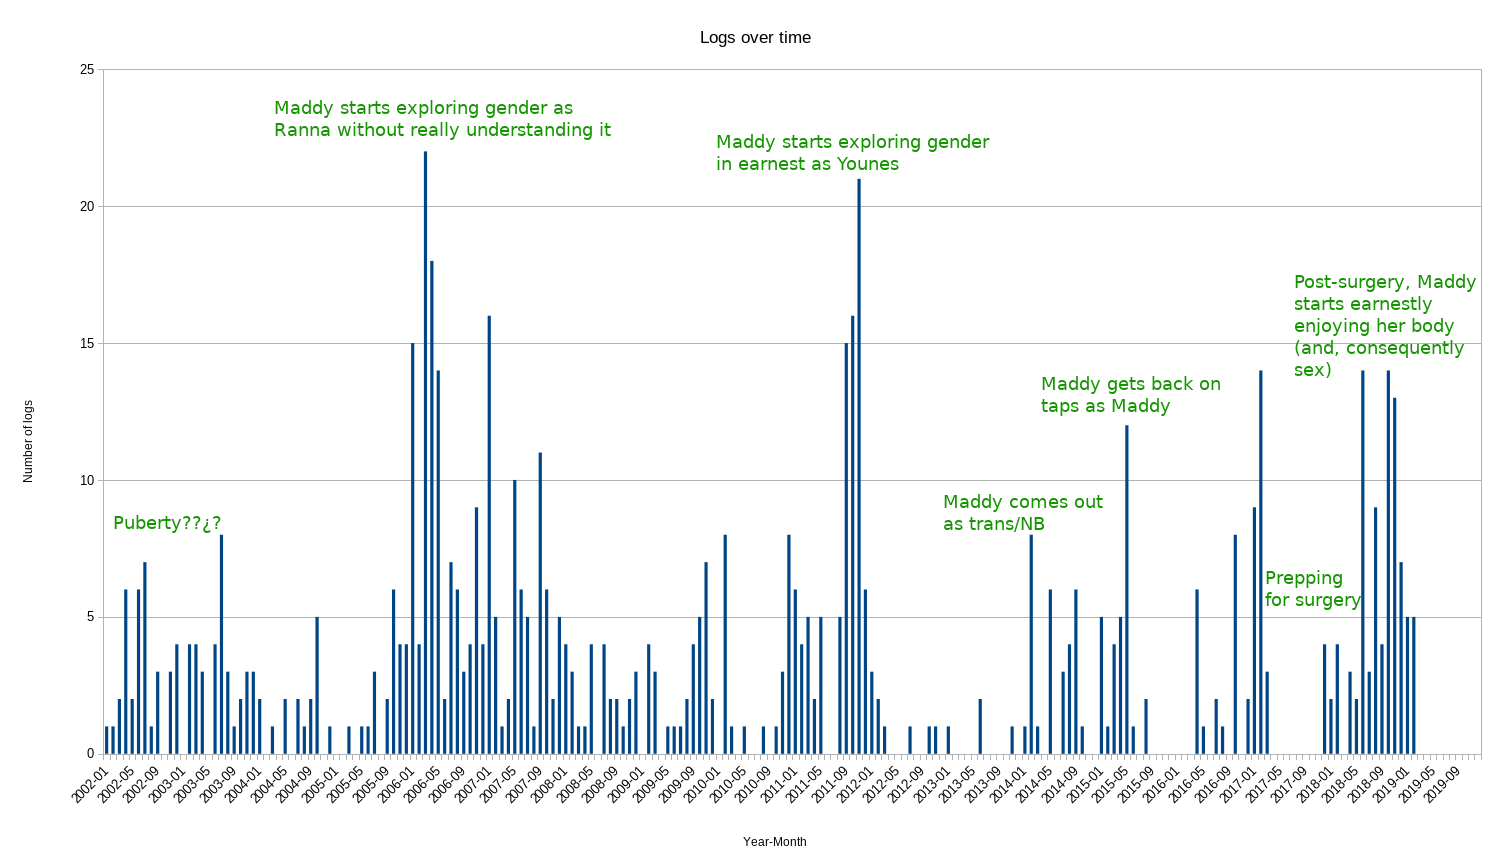
\includegraphics{/ts-graph.png}}

\begin{ally}
You are a parody of yourself.
\end{ally}
And proud of it.
\newpage

So, I think the order of my entry to furry was as follows:

\begin{enumerate}
\def\labelenumi{\arabic{enumi}.}
\item
  Find a furcode in someone's forum sig.

  \begin{ally}
  Oh my aching bones.
  \end{ally}
  Shut up, you're not that old, the internet just moves \emph{really} fast. Besides, you don't have bones.
\item
  Find a furcode decoder.
\item
  Find Captain Packrat's page on furry.
\item
  Find Yerf!.
\item
  Make a dragon character.
\item
  This lasts three days. No one pays attention to me. Make a fox character.
\item
  Meet some furries on GovTeen (née Puberty101).
\item
  Start talking with furries on AIM.
\item
  Join FluffMUCK.
\end{enumerate}

\begin{ally}
Ah yes, Fluff. May she rest in eternal solitude.
\end{ally}
She's not totally gone. I don't think. I actually haven't checked in a while.

\begin{ally}
I'm starting to doubt your commitment to nostalgia, here.
\end{ally}
What would I gain from such?

\begin{ally}
You could go look in the park. You could go ride around in the Universe-in-a-Box. You could \texttt{laston} some folks, maybe.
\end{ally}
Weirdly enough, of the people I would \texttt{laston}, I was finally reintroduced to a few not too long ago by, of all people, Zorin, head wiz of Fluff. Rela and GC. I was glad to see them doing well.

\begin{ally}
You were glad to see they were alive.
\end{ally}
I was glad to see they were alive, yes. That was around the time I had found the obituary for Danny.

\begin{ally}
You could \texttt{laston} Marek.
\end{ally}
I'm not sure I could take that.

\begin{ally}
Is that why you don't want to connect?
\end{ally}
It's one reason. Nostalgia is only so much fun. It's fun up until a certain extent, and then it becomes painful.

\begin{ally}
It's fun up until you're confronted with mortality and uncertainty. Danny died, and you don't know if Marek's alive.
\end{ally}
Yeah.

It's no longer fun, but it's no less important.

\begin{ally}
Let's talk about Margaras.
\end{ally}
Not yet.

\begin{ally}
Danny's passing was an abstract thing. Maragaras' was much more immediate. Much more concrete and real.
\end{ally}
Please.

\begin{ally}
Take your time.
\end{ally}
\newpage

The first furry I met, aside from Ash, was Osric. We went to see a movie. We were so painfully shy.

\begin{ally}
After seeing the movie, you drove him back to where he had parked, and you sat for a few moments in pained silence, then hugged and went your separate ways.
\end{ally}
Years later, I'd take a picture of him and his husband after his graduation that I think they still have. Years after that, his husband would officiate JD and I's wedding.

\begin{ally}
When was the last time you talked with either of them?
\end{ally}
Bel favorited a tweet of mine not too long ago.

\begin{ally}
You grew up.
\end{ally}
Yeah, we all grew up. We bought houses. We got jobs.

JD and Os dated for a little, and Bel and I nearly did. Even up until when I was working on polycul.es, we had dashed lines between us. I loved them.

\begin{ally}
`Loved'?
\end{ally}
I still do. Very much so. But every year, that love gets more abstract. More academic.

Bel and I clicked on a sexual and nerdy level on which Os and I seemed to miss each other. I wasn't toppy enough for Os, and the nerdery --- minus, briefly, EVE --- was work, for him.

\begin{ally}
Eventually, it got that way with you, too. And then you started feeling uncomfortable with sex.
\end{ally}
Our relationships were organic. We met randomly. We drifted closer, orbited each other, and then we drifted apart. The same happened with friends from high school and university. The same happened with friends from the PN on FurryMUCK.

From those first, halting meetings, I wound up slowly working my way into meeting furries in person. First, there were the few at school. Then the few at the queer group. Then, in university, Os dragged me to Fort Fur Friday, which I attended basically until they moved out of Fort Collins. That's where I met JD.

Then I managed to make it to Anthrocon 2005. Then Further Confusion 2007. I was sold.

There's this trope that pokes its head up every now and then, that there is an age-out date for furry. A time when you realize you're too old for this shit and peace.

\begin{ally}
When I was a child, I talked like a child, I thought like a child, I reasoned like a child. When I became a man, I put the ways of childhood behind me.
\end{ally}
There is some of that, yes, but I like Qoheleth more than Paul. I like Ecclesiastes better than the epistles.

\begin{ally}
When you graduated high school, you stamped I Cor. 13 in your friends' yearbooks.
\end{ally}
When I was a child, I talked like a child, I thought like a child, I reasoned like a child. When I became a man, I put the ways of childhood behind me.

\begin{ally}
Well played.
\end{ally}
There is a time for reaping and a time for sowing; there is a time for being a hardcore nutjob furry and a time for taking a break and just being a human for a while.

\begin{ally}
This, too, is meaningless.
\end{ally}
Well played.
\newpage

A time to kill, and a time to heal; a time to break down, and a time to build up.

My interest in furry wound down a bit in university. I'd burned myself a bit too hard, hurt too many people, grew too jaded to take part. I still prowled around the usual haunts on the MUCKs, still poked my head in FFF, still looked at all the art, \href{https://adjectivespecies.com/2012/03/21/makyos-kaddish/}{but my heart wasn't in it anymore}.

\begin{ally}
There was a reason behind this. There were people behind this.
\end{ally}
Well, true. I don't know how to square that with\ldots{}well, a lot of things.

\begin{ally}
You don't know how to square that with how you felt about those people at the time.
\end{ally}
That's one aspect, yes. I also don't know how to square that with the fact that I was growing too jaded in a lot more than just furry. I grew jaded at school. I grew jaded at work. I struggled with my relationships. I struggled.

\begin{ally}
You struggled with gender.
\end{ally}
Well, yes, but I wasn't quite ready to admit that, yet.

\begin{ally}
You struggled with self harm.
\end{ally}
Yes.

\begin{ally}
You struggled with the intersections, the interstices, and the liminal spaces.
\end{ally}
I was going to write about {[}a{]}{[}s{]}. Where are you taking me?

\begin{ally}
Straight homeward to your symbol-essences.
\end{ally}
Shall I not die, then?

\begin{ally}
Isn't that the point of writing?
\end{ally}
I'm pretty sure all our names are writ on water at this point.

\begin{ally}
Come now. You wanted to be Keats when you grew up.
\end{ally}
You're in a mood.

\begin{ally}
You're in a mood.
\end{ally}
Fine.

Where are you taking me?

\begin{ally}
Let {[}a{]}{[}s{]} speak for {[}a{]}{[}s{]}. Let yourself speak for yourself.
\end{ally}
Okay.
\newpage

\begin{ally}
Who are you?
\end{ally}
I'm Madison Jesse Scott-Clary.

\begin{ally}
What are you?
\end{ally}
I\ldots{}what?

\begin{ally}
Who are you?
\end{ally}
I answered you.

\begin{ally}
Tell me your names.
\end{ally}
I am Madison. I am Maddy. I am Makyo.

\begin{ally}
No Sarai? No Happenstance, or Younes?
\end{ally}
Sarai could die. I couldn't be her. Happenstance was a coping mechanism for gender. Younes was\ldots{}

\begin{ally}
Tell me about Younes, then. That's where you started going before, right?
\end{ally}
Yeah, though you've certainly changed the tenor of it. The mood.

\begin{ally}
No one said this project would be easy.
\end{ally}
\newpage
